\chapter{Introduction}
\section{Overview of Scene}


\subsection{Background}
%\paragraph{This paragraph denotes what I struggled to include in the final source code. }
\subparagraph{"In keeping with the theme of a futuristic emerald isle, I created a dystopian world where humanity has been forced underground to escape rising temperatures due to global warming. Individuals are reminded of the impending doom as they look up to see a black hole, actively swallowing planets!
In the scene we can see how humanity has been forced to innovate, taking over stalactite structures and using them as buildings. Materials used to build these was recently discovered and is ultra high-tec!"}



\subsection{Implementations}
\paragraph{This paragraph denotes what was achieved in the final source code. }
\subparagraph{

Several complex features were required to be implemented as detailed above. Below is a comprehensive list of what I achieved.}

\subparagraph{
I successfully rendered and textured buildings, roads and other objects for my scene. A custom SkyBox was put together and implemented correctly using online free use images and Adobe Editor. Camera control was included to allow user interaction with the scene. 

A point light source and lighting were attempted but incorrectly implemented and had to be scrapped. Animation was also attempted but couldn't be included in the scene. The MP4 video and screenshots show these implementations/ attempts.

The frame rate is steadily above 15 FPS as shown in MP4.}

\subsection{Challenges}
\subparagraph{This paragraph denotes what I struggled to include in the final source code. }
\paragraph{Unfortunately not all of the requirements for the project were met. Below is a comprehensive list of what I struggled to do.

I began working on an infinite plane but struggled to complete a chunking method. Upon defining a plane struct as well as reshaping my shaders to clamp the eye in place, I saw strange results. The camera was being reset, but any input lead to 'shaking'. This was omitted as a result.

I found lighting and shadows particularly difficult to implement. See below for my best attempt. I was able to define the logic for lighting and shadow creation in my shaders, however I could not integrate this with my texture mapping. Debugging attempts included binding the textures at earlier points in the runtime, ensuring correct UV Buffer, texCoords passed between shaders, etc. Unfortunately I could not figure this out and lighting had to be omitted. The code is still available on the Git repository.

Animation also had to be omitted for similar reasons. I was seeing positive results (skeleton runs as expected, no errors), but when included in the render loop, the rest of the scene disappeared. I believe this is due to some reassigning of OGL parameters.

}

\subparagraph{
\begin{figure}
    \centering
    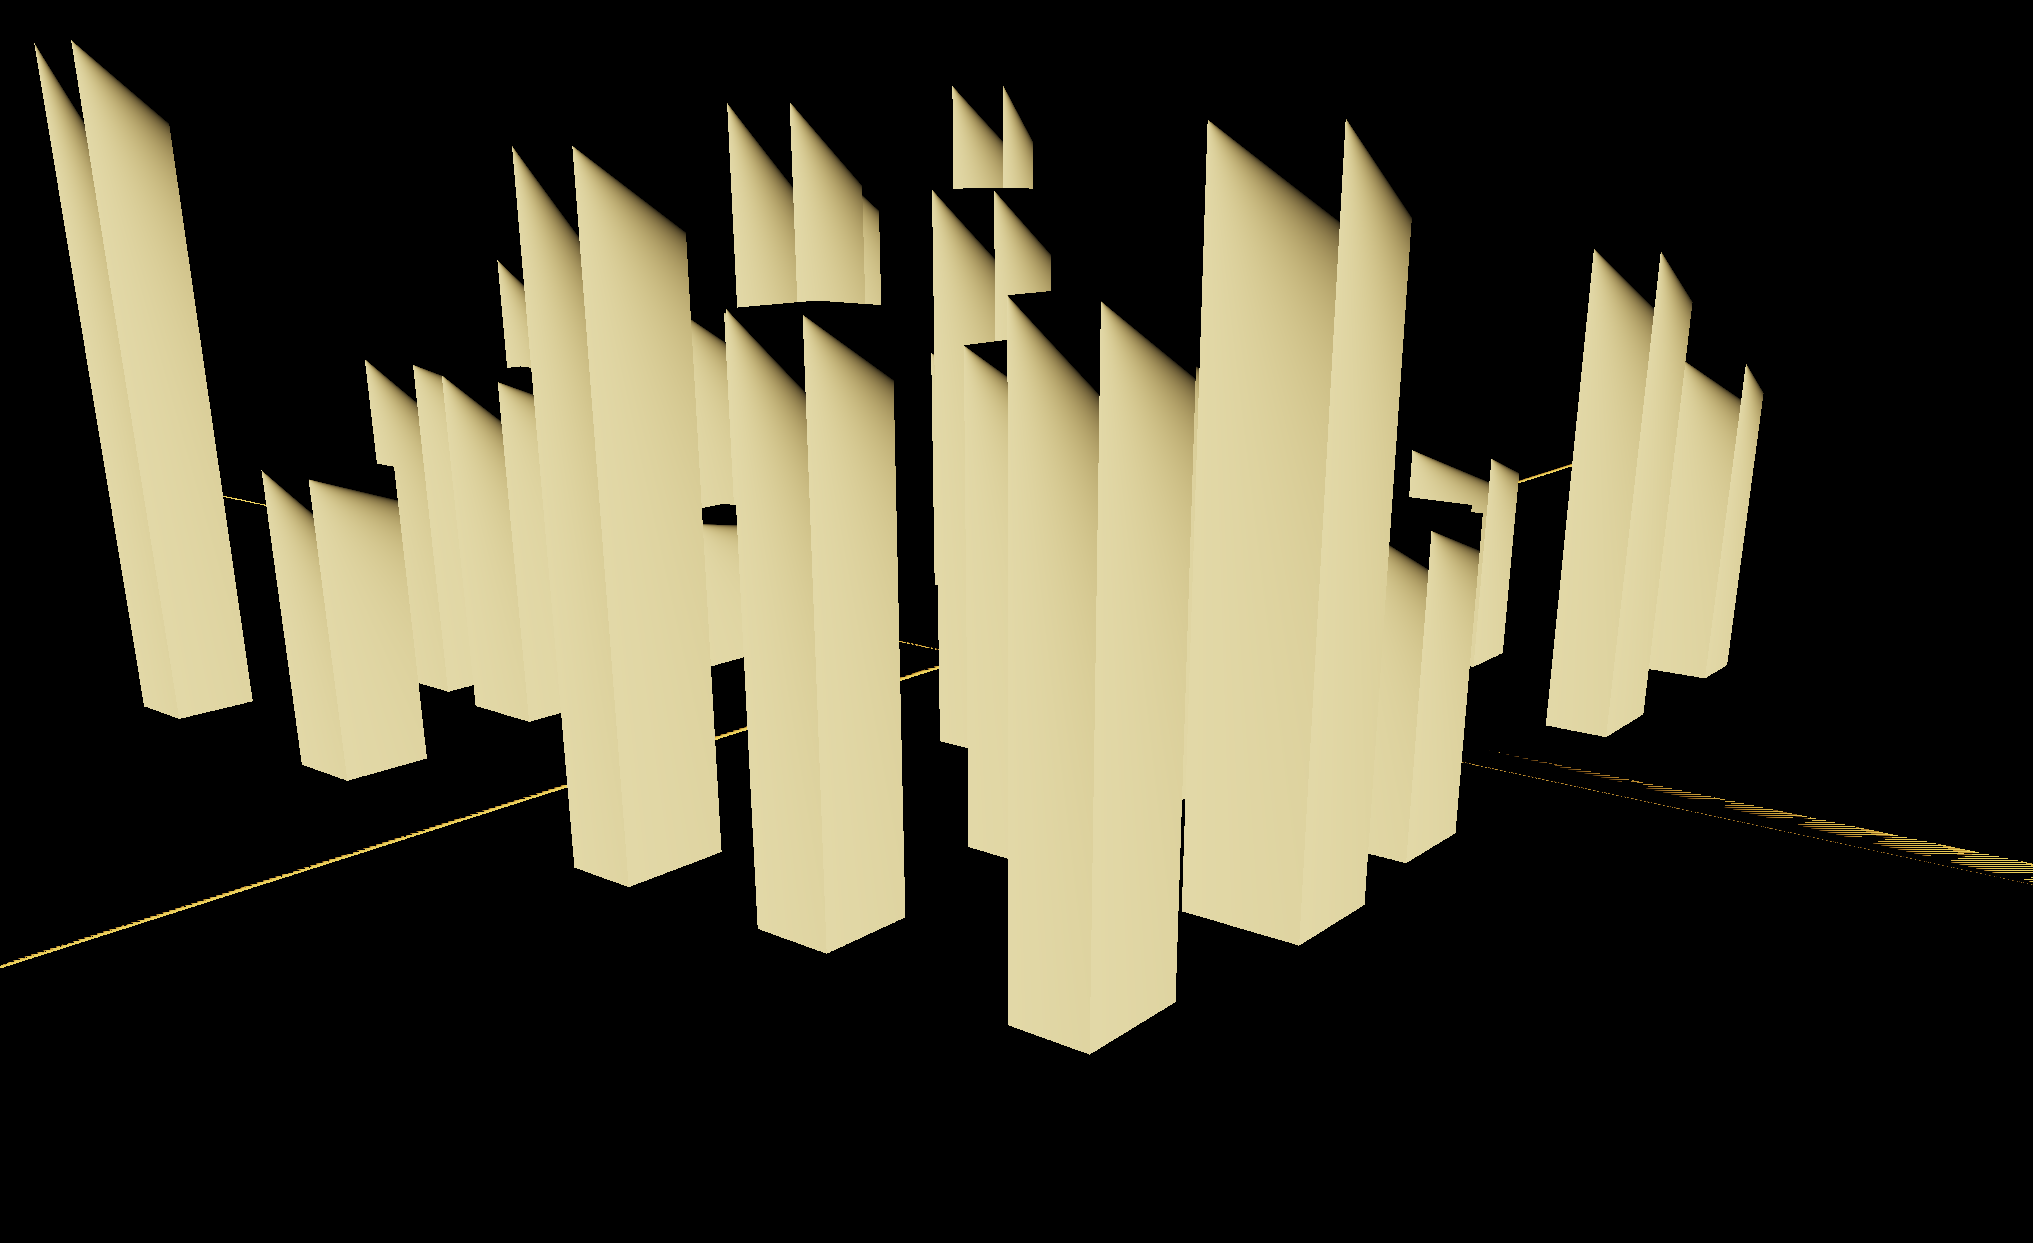
\includegraphics[width=0.5\linewidth]{Results//Progress_screenshots/Screenshot 4 - Lighting & Shadows Attempt.png}
    \caption{Attempting lighting and shadows}
    %\label{fig:enter-label}
\end{figure}

}
